\documentclass{article}

\usepackage{pgf}
\usepackage{tikz}
\usetikzlibrary{arrows, automata}
\usepackage[latin1]{inputenc}
\usepackage{verbatim}

\begin{document}

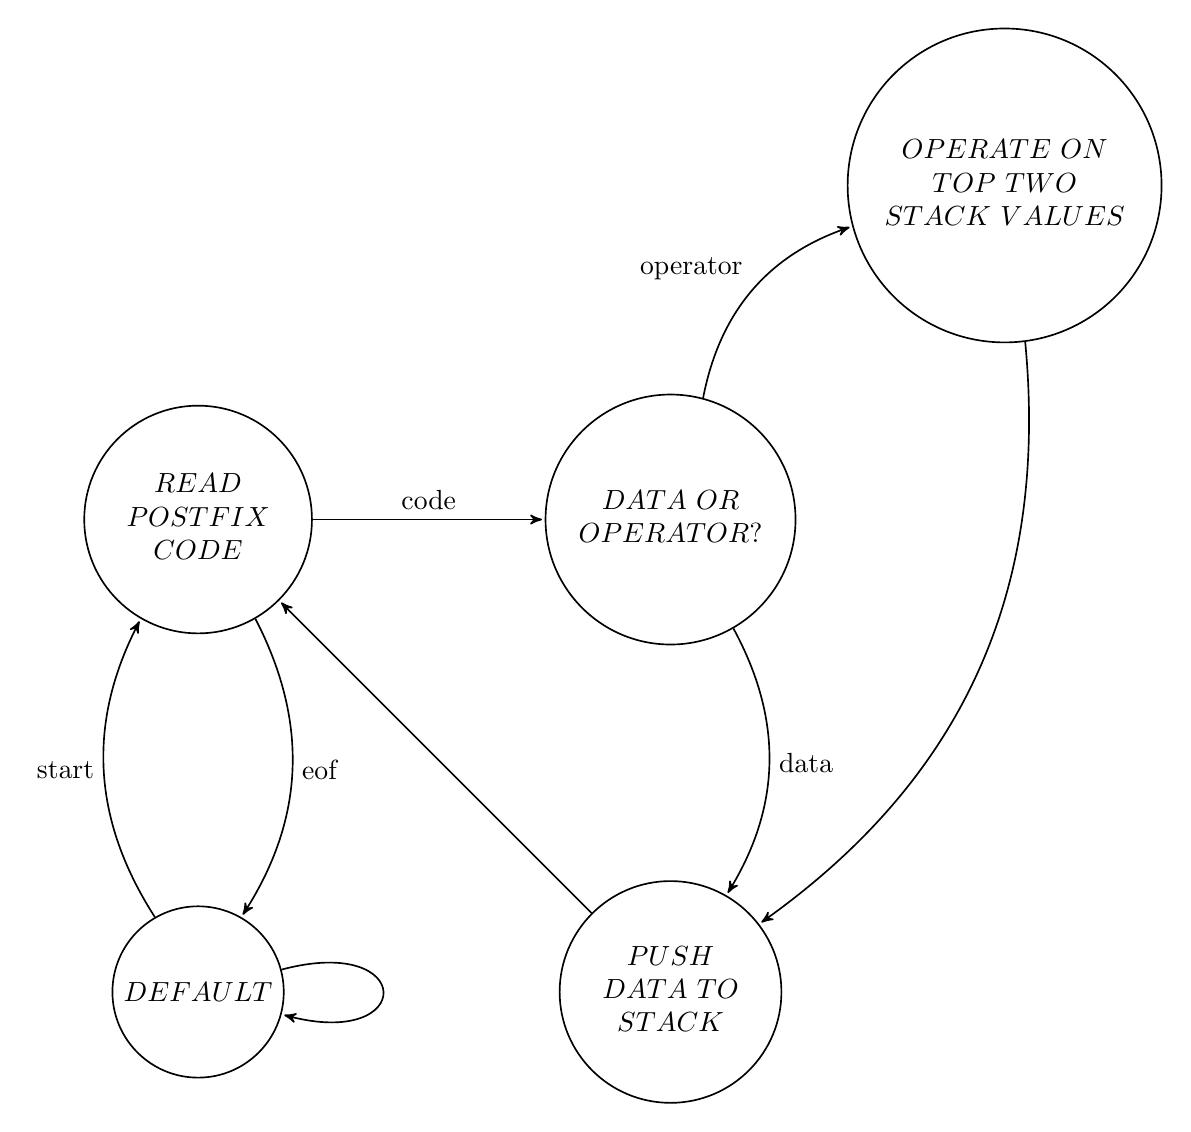
\begin{tikzpicture}[->,>=stealth',shorten >=1pt,auto,node distance=6cm, semithick]
  \tikyle{every state}=[draw=none,text=black]

  \node[state] (A)                         {$DEFAULT$};
  \node[state] (B) [above of=A]            {\begin{tabular}{c}$READ$\\$POSTFIX$\\$CODE$\end{tabular}};
  \node[state] (C) [right of=B]            {\begin{tabular}{c}$DATA\ OR$\\$OPERATOR?$\end{tabular}};
  \node[state] (D) [below of=C]            {\begin{tabular}{c}$PUSH$\\$DATA\ TO$\\$STACK$\end{tabular}};
  \node[state] (E) [above right of=C]      {\begin{tabular}{c}$OPERATE\ ON$\\$TOP\ TWO$\\$STACK\ VALUES$\end{tabular}};

\path

(A) edge [loop right] node {} (A)
(B) edge             node {code} (C)
(B) edge [bend left] node {eof} (A)
(C) edge [bend left] node {data} (D)
(C) edge [bend left] node {operator} (E)
(E) edge [bend left] node {} (D)
(D) edge [] node {} (B)
(A) edge [bend left] node {start} (B);

\end{tikzpicture}
\end{document}